\chapter{Appendix}

\section{Mathematical Notation}
\label{sec:app:mathnot}
For simplicity, any physical unit will be abstracted here by the arbitrary function $f(\xi)$.
The notation for this thesis has been defined as follows: 
\subsection{Vectorial and Scalar Units}
Vector or tensor symbols are written in bold font, while normal font is used for scalar units. Forces - independently of magnitude or direction - are shown with a bold, capital $\mathbf{F}$. The imaginary unit is connoted as $i$.\\ Normal acting properties are multiplied with the \acrfull{surfnormal}. The normal vector to a plane spanned by two independent vectors is calculated by the cross-product $f \times f$, while the scalar product is denoted by the centered dot $f \cdot f$.
\subsection{Differential Operators}
In the derivations, following after \cref{eq:continuityP,eq:conservMass}, the gradient operator is symbolized by $\nabla f$. The divergence operator of an arbitrary function $f$ is utilized as $\nabla\cdot f$. The Laplace operator, in scalar context known as the second order derivative, is generalized here as $\nabla^2 f$ and equals $(\nabla\cdot\nabla) f$ respectively. It should be not confused with the capital delta $\Delta$, which indicates the difference of a unit, such as $\Delta f = f{2} - f{1}$. The identity matrix $\mathbf{I}$ is indexed by its size, for example $\mathbf{I}_{\scaleto{3 \times 3}{4pt}}$. 

\begin{align}
	\sum_{i} f(\xi = i)&= \sum_{i = 0}^{\infty} f(\xi = i) \label{eq:app:sum}\\
	\int_{a}^{b} f(\xi) \mathrm{d\xi} &= F(b) - F(a) \label{eq:app:intDef}\\
	\int f(\xi) \mathrm{d\xi}&= F(\mathrm{\xi}) + c \label{eq:app:intIndef}
\end{align}

\subsection{Integration and Summation Operators}
The index of an infinite sum is shown in \cref{eq:app:sum}  and starts at \num{0} unless specified otherwise. If the boundaries of an integral are not shown at the top and bottom (\cref{eq:app:intDef}), it is considered as indefinite integral (\cref{eq:app:intIndef}) with the integration constant $c$. However, $c$ denotes during the course of this work - due to a lack of explicitly solved integrals - concentrations.
For surfaces and volumes, the integral is repeated according to the respective dimension. In the indefinite case, the unit surface is denoted by $\mathrm{dA}$, and in the volumetric case by $\mathrm{dV}$. 

\subsection{Equations and Inequalities}
Approximated or estimated units are expressed by an equal sign with the assumption in overset or two tildes above each other. For sufficiency conditions, mostly inequalities were used. In these, double angular brackets, $\ll$ or $\gg$, imply an value difference of at least one order of magnitude. Postulated conditions are indicated by an exclamation mark above the equal sign: $\overset{!}{=}$.

\clearpage
\section{Additional Figures}
\begin{figure}[h!]
	\centering
	\subfloat{
		\subfigimg[clip,trim=115 100 80 60, height=95pt]{a}{./Ressources/Fluidic/Transient_SyringePump.jpg}
		\phantomsubcaption
		\label{fig:fluidic:pumpStability:transient}
	} \hfill 
	\addtocounter{subfigure}{-1}
	\subfloat{
		\subfigimg[height=95pt]{b}{./Ressources/Fluidic/SyringeSteadyState.eps}  
		\phantomsubcaption
		\label{fig:fluidic:pumpStability:steadystate}
	}
	\capption{Syringe Pump error sources}{Set flow rate: \orangeline, Real Flow Rate: \blueline. The transient term of the \gls{nse} (\cref{eq:navierstokes}) was neglected in all simulations. However, a connected syringe pump retains a finite rise time (\textbf{a}) and a remaining ``pulsation error'' in steady state (\textbf{b}). In effect, an error adds to simulation and experiment. Therefore, any measurement can only be valid several ten seconds after the last flow rate change. (\textbf{a}) Exemplary, transient step answer of a syringe pump through a microtube with \SI{254}{\micro\meter} inner diameter. (\textbf{b}) Steady state flow rate error around the desired \SI{5}{\micro\liter\per\minute} dispensing rate. A sinusoidal behavior caused by the microstepping can be observed. \cite{lit:fluidic:fluigentPumpStability}}
	\label{fig:fluidic:pumpStability}
\end{figure}


\begin{figure}[h!]
	\centering
	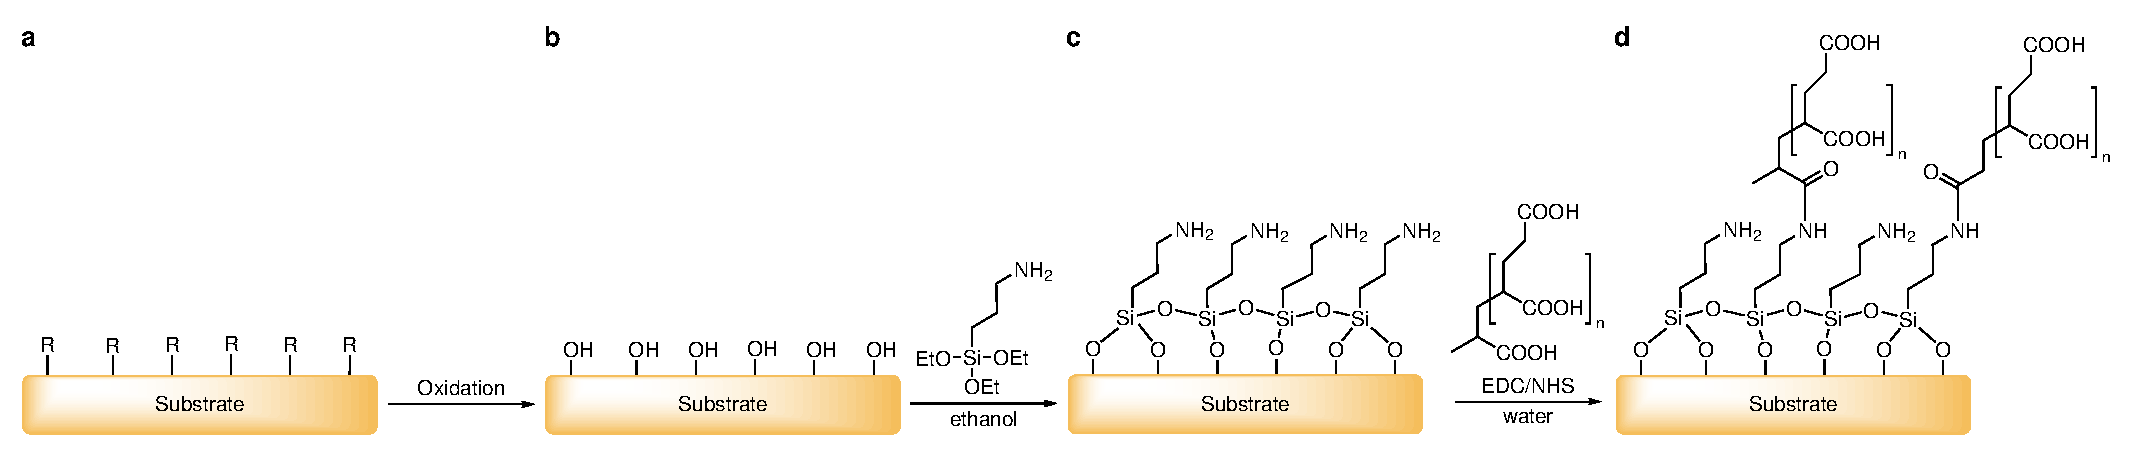
\includegraphics[width=1\linewidth]{Ressources/Chemistry/Substrate}
	\capption{General process chain of chemical surface modification}{Any substrate with various surface groups R (\textbf{a}) is oxidized to exhibit \gls{hydroxyl} groups.(\textbf{b}). Then a silane \gls{sam} is attached (\textbf{c}) and subsequently modified by carbodiimide chemistry with \gls{paa}. (\textbf{d})}
	\label{fig:chem:func:withPAA}
\end{figure}%\todo{größer, schöner}

\begin{figure}[!h]
	\centering
	\subfloat{
		\subfigimg[height=150pt]{a}{Ressources/Differential/Bottom}	
	} \hfill
	\subfloat{
		\subfigimg[height=150pt]{b}{Ressources/Differential/Top}	
	}
	\capption{Flow Rate Dependency of Differential Counting Setup}{(\textbf{a}) Optimized for top sensor (\textbf{b}) Optimized for bottom sensor}
	\label{fig:diff:flowRate}
\end{figure}

\begin{figure}[!h]
	\centering
	\includegraphics[width=.3\linewidth]{Ressources/Concentration/CaptureVelocity}
	\capption{Measured Bead Velocity}{ Not sure what to say about velocity itself. Maybe remove completely,   p < 0.01}
	\label{fig:conc:vel}
\end{figure}

\begin{figure}[!h]
	\centering
	\includegraphics[height=150pt]{Ressources/ResultPlots/PDMS-sessileDrop}
	\capption{Hydrophobicity Analysis of \gls{pdms} under Plasma Exposure}{For an optimal plasma bond to glass, \gls{sin} and \gls{pdms}, the contact angle was measured after treatment. The initial decrease until \SI{45}{\second} declares the optimum around this time. Longer times should be avoided consequently to prohibit further surface damages by reactive ions. }
	\label{fig:coval:plasma}
\end{figure}

